\documentclass{beamer}
\usepackage{hyperref}
\usepackage{xcolor}
\usepackage{graphicx}
% Theme choice:
\usetheme{Madrid}

% Title page details: 
\title{Modelo predictivo del crecimiento poblacional} 
\subtitle{Equipo \#2}
\author{\textit{Estimación de la capacidad de carga }}
\date{\today}
\logo{\large \LaTeX{}}

\begin{document}

% Title page frame

\begin{frame}
    \titlepage 
    \underline{\textbf{Integrantes: }}\\
    Guillermo Cepero García \\ Luis Ernesto Serras Rimada \\ Miguel Vadim Vilariño Pedraza
\end{frame}

% Remove logo from the next slides
\logo{}
\author{\textit{\underline{\textbf{Equipo \#2}}}}

\section{Introducción}
\begin{frame}{El crecimiento poblacional}
    \begin{center}
        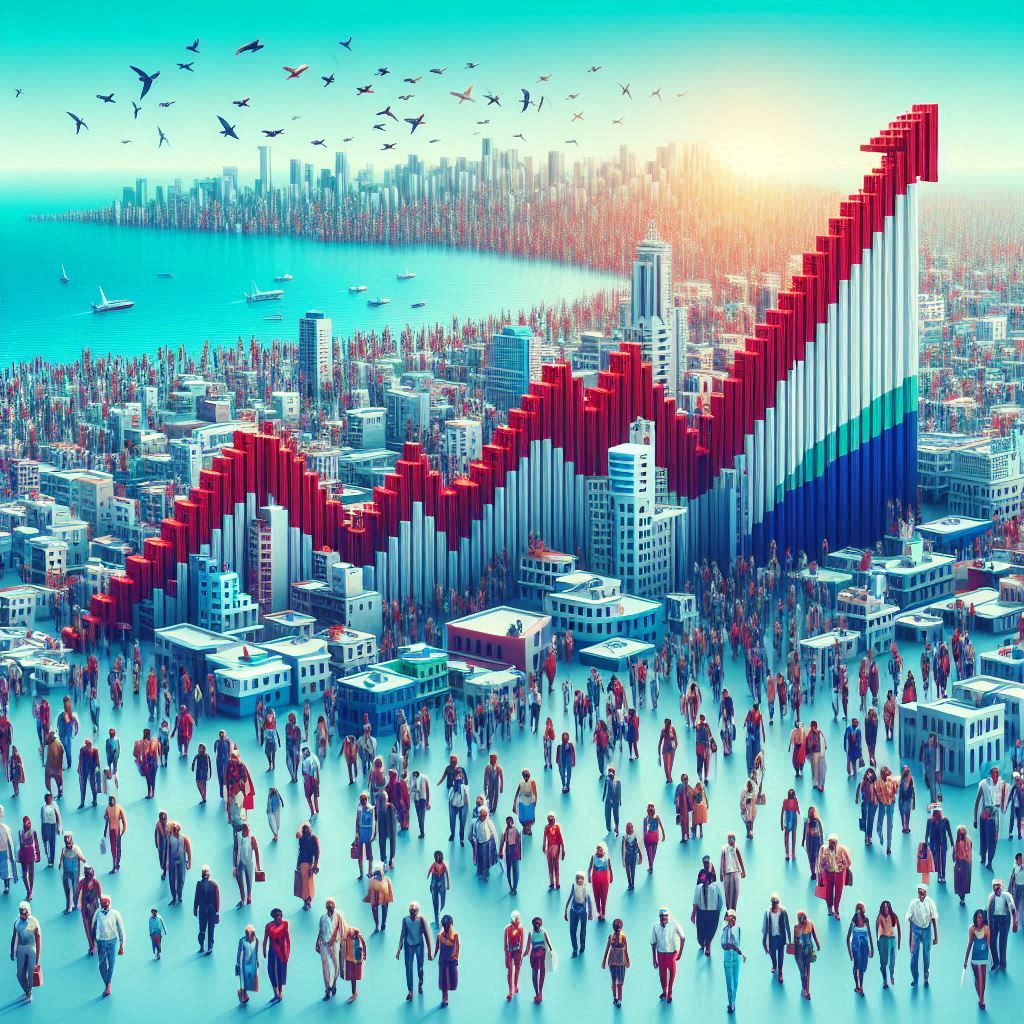
\includegraphics[height = 5cm]{img/cuba1.jpeg}
        \\
        \small{El análisis del crecimiento poblacional reviste gran importancia debido a su relevancia en diversos campos como la economía, demografía, epidemiología, la ecología, entre muchos otros. Resulta útil en múltiples ámbitos, incluyendo estudios demográficos, planificación urbana y análisis de recursos naturales. Conocer un resultado aproximado que se
        acerque a una solución real del crecimiento poblacional permitiría beneficiar significativamente la dirección y gestión de recursos en nuestro país.}    
    \end{center}
\end{frame}

\begin{frame}{Crecimiento poblacional en Cuba}
    \small{Según datos de la Oficina Nacional de Estadísticas e Información de Cuba (ONEI), la población del país aumentó de aproximadamente 6.5 millones en 1953 hasta alcanzar un máximo de 11.2 millones en 2016. Desde entonces, ha experimentado una ligera disminución, llegando a los 11.0 millones en 2022.}
    \begin{block}{\small{Las causas principales de este patrón de crecimiento han incluido factores como: }}
    \begin{itemize}
        \item \small{La política socialista de Cuba (que priorizó la educación y la salud pública, lo que llevó a un aumento en la esperanza de vida y la reducción de la mortalidad infantil)}
        \item \small{Las migraciones internacionales (especialmente desde la década de 1990)}
        \item \small{Los cambios en las políticas familiares, como la legalización del aborto y la anticoncepción, que afectaron la fertilidad de la población.}
        \item \small{Y el impacto de la crisis económica de 1991, que llevó a un cambio en las actitudes hacia la planificación familiar; entre otros. }
    \end{itemize}
    \end{block}
\end{frame}
\begin{frame}{Objetivos}
    Por ende, los objetivos principales de este análisis son:\\
\begin{itemize}
    \item Estimar el número máximo de personas que pueden ser sostenidamente alojadas en un área geográfica determinada y evaluar el equilibrio entre la población existente y la capacidad de carga ambiental
    \item Contribuir al diseño de estrategias de planificación urbana y rural que equilibren el crecimiento económico con la protección del medio ambiente y los servicios básicos.
    \item Permitir evaluar el impacto potencial del cambio climático y otros factores externos en la capacidad de carga poblacional a largo plazo.
    \item Contribuir al diseño de programas de educación ambiental y concientización sobre las implicaciones del crecimiento poblacional.
    \item Ayudar a establecer límites razonables para el crecimiento demográfico, evitando excederse en la explotación de recursos naturales y servicios públicos.
\end{itemize}

\end{frame} 

\section{Ecuación Diferencial}
\begin{frame}{Modelo logístico}
    Se plantea trabajar el asunto con un modelo matemático que nos pueda conducir a dicha prediccion, y se considera 
    el \textbf{modelo del crecimiento logístico}, que es solución de la ecuación diferencial que describe cómo la tasa de crecimiento de la población (dP/dt) 
    cambia con el tamaño de la población (P(t)) 
    \begin{block}{Ecuación Diferencial:}
    $$\frac{dP}{dt} = r \cdot P(t)(1 - \frac{P(t)}{K}) $$
    \end{block}
\end{frame}
\begin{frame}{Parámetros a estimar}
\begin{block}{Donde se tiene que:}
\begin{itemize}
    \item (P(t)) es la población en función del tiempo (t).
    \item (r) es la tasa de crecimiento intrínseca de la población.
    \item (K) es la capacidad de carga o tamaño máximo sostenible de la población.
\end{itemize}
\end{block}

\begin{block}{Parámetros a Estimar:}
\begin{itemize}
    \item (r): Tasa de crecimiento intrínseca de la población. 
    \item (K): Capacidad de carga de la población.
\end{itemize}
\end{block}
\end{frame}

\section{Modelo Matemático}
\begin{frame}{Modelo del crecimiento logístico}
    \begin{block}{La ecuación tiene la forma: }
    $$P(t) = \frac{K}{1 + Ae^{-rt}}$$
    Y para encontrar (A) es:
    $$P(0) = \frac{K}{1 + Ae^{0}}$$
    \end{block}
    Nota: \textbf{(A)} es una constante que depende de las condiciones iniciales de la población.
\end{frame}

\begin{frame}
    Esta función muestra claramente el punto de inflexión, donde la tasa de crecimiento cambia de positiva a negativa, indicando que la población 
    ha alcanzado su capacidad de carga y está comenzando a estabilizarse.
\begin{center}
    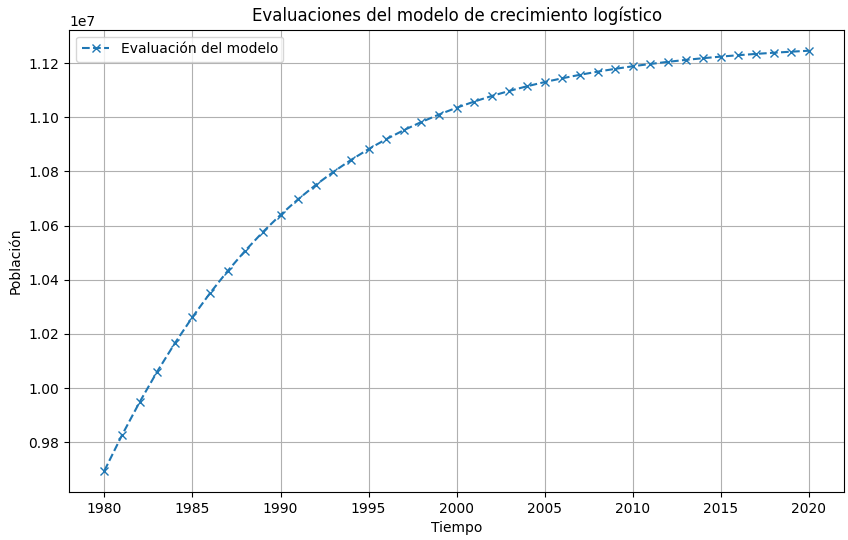
\includegraphics[height= 6cm]{img/model.png}
\end{center}
\end{frame}

\section{Implementación en Python}
\begin{frame}{curvefit}
    Se utilizaron los datos históricos de densidad poblacional desde 1980 hasta 2020 publicados en las series estadísticas del sitio web de la ONEI. Y se desean ajustar los parámetros de la capacidad de carga($K$) y la tasa ($r$).
    Para ello se decide utilizar la aproximación por mínimos cuadrados por medio de la función curvefit del módulo scipy.optimize en Python, cuya función matemáticamente se puede representar como:\\
    Minimizar: $\sum_{i=1}^{N} (y_{i} - f(x_{i}, \theta))^2 $ \\
    \begin{block}{Y toma los parámetros:}
    \begin{itemize}
        \item f: es la función modelo para la optimización.
        \item xdata: son los valores independientes (el tiempo ($t$ como $x_{i}$)).
        \item ydata: son los valores dependientes (los valores de densidad poblacional en función del tiempo ($P$ como $y_{i}$)).
        \item p0: Estimación inicial.
    \end{itemize}
    \end{block}
\end{frame}

\begin{frame}
    \small{La función curvefit intentará minimizar la suma de los cuadrados de los residuales para encontrar los valores óptimos de $K$ y $r$ que minimizan esta expresión.} \\\\
    \textbf{Paso 1: Definición de la Función de Pérdida:\\}
    \small{El objetivo es minimizar la suma de los cuadrados residuales, que es la suma de las diferencias cuadradas entre los valores de la población observada (Pdata) y los valores de la población ajustados (f(tdata, K, r)).\\}
    \begin{block}{Suma de cuadrados residuales:}
        $$\sum_{i=0}^{N}[(Pdata(t_{i}) - f(tdata_{i}, K, r))^2]$$
    \end{block}
    \textbf{Paso 2: Inicialización de los Parámetros:}\\
    Se proporcionan valores iniciales para los parámetros K y r (initial-guess).\\
\end{frame}

\begin{frame}
    \textbf{Paso 3: Iteración hacia los Parámetros Óptimos:}\\
    \small{La función curve-fit utiliza el algoritmo de \textbf{Levenberg-Marquardt} para encontrar los valores de K y r que minimizan la suma de cuadrados residuales. Este algoritmo iterativo implica los siguientes pasos:}
    \begin{enumerate}
        \item \small{Cálculo de la matriz $\omega$: Se calcula de la función de pérdida, la matriz $\omega$ que contiene las derivadas parciales de la función de pérdida con respecto a los parámetros K y r.}
        \item \small{Actualización de Parámetros: Utilizando la matriz $\omega$, se calculan nuevas estimaciones para K y r que minimizan localmente la función de pérdida.}
        \item \small{Repetición: Los pasos 1 y 2 se repiten hasta que se alcanzan los criterios de convergencia (por ejemplo, un cambio insignificante en los parámetros o un número máximo de iteraciones).}
    \end{enumerate}
\end{frame}
\begin{frame}{Calculo de la matriz $\omega$}
    $\omega$ es una matriz que contiene las derivadas parciales de la función de pérdida con respecto a los parámetros K y r.
    \begin{block}{Se calcula como: }
        $$\omega = [\frac{\delta(r_{min})}{\delta(K)}, \frac{\delta(r_{min})}{\delta(r)}]$$
        
        \begin{center}\small{siendo $r_{min}$ la suma de cuadrados residuales}\end{center}
    \end{block}
    Donde f(tdata, K, r) es la función logística:
    \begin{block}{Se tiene la función de pérdida:}
    $$f(t, K, r) = \frac{K}{(1 + ((\frac{K}{P_{0}}) - 1)e^{-rt})}$$
    donde $P_{0}$ es el valor inicial de la población en el período de tiempo. 
    \end{block}
\end{frame}

\begin{frame}{Derivadas Parciales}    
\small{Para calcular las derivadas parciales, diferenciamos la función de pérdida con respecto a K y r.\\}
\begin{block}{Derivada parcial con respecto a K:}
$$\omega = \frac{\delta(r_{min})}{\delta(K)} = \sum_{i=0}^{N}[2(P(t_{i}) - f(tdata, K, r)) \cdot (\frac{-f(tdata, K, r)}{K^{2}})]$$
\end{block}
\begin{block}{Y sustituyendo  f(tdata, K, r) en la derivada, obtenemos:}
    $$\omega = \frac{\delta(r_{min})}{\delta(K)} = -2\sum_{i=0}^{N}[(P(t_{i}) - \frac{K}{(1 + ((\frac{K}{P_{0}} - 1) \cdot e^{-r \cdot t})) \cdot (\frac{K}{(1 + ((\frac{K}{P_{0}} - 1) \cdot e^{-r \cdot t}))})^{2}})]$$    
\end{block}
\end{frame}

\begin{frame}  
\begin{block}{Derivada parcial con respecto a r:}
$$\omega = \frac{\delta(r_{min})}{\delta(r)} = $$ 
\small{$$=\sum_{i=0}^{N}[2(P(t_{i}) - f(tdata, K, r)) \cdot (f(tdata, K, r) \cdot \frac{(\frac{-K}{P_{0}}) \cdot e^{-rt}}{(1 + ((\frac{K}{P_{0}} - 1) \cdot e^{-rt})^{2})})]$$}
\end{block}
\begin{block}{Y sustituyendo  f(tdata, K, r) en la derivada, obtenemos:}
$$\omega = \frac{\delta(r_{min})}{\delta(r)} = $$
\small{$$= -2\sum_{i=0}^{N}[(P(t_{i}) - \frac{K}{(1 + ((\frac{K}{P_{0}}) - 1) \cdot e^{-rt})} \cdot \frac{K}{(1 + ((\frac{K}{P_{0}}) - 1) \cdot e^{-rt})^{2}}) \cdot (\frac{-K}{P_{0}}) \cdot e^{-rt}]$$}
\end{block}
Evaluando estas derivadas en los valores iniciales de K y r, obtenemos $\omega$
\end{frame}

\begin{frame}{Ecuación normal}
    Luegp se forma una ecuación normal utilizando $\omega$ y la matriz de Hessiana (H), que es la matriz de segundas derivadas parciales de la función de pérdida. La ecuación normal es:
    $$(\omega^{T}\omega + \lambda I)\triangle p = -\omega^{T} r$$
    \begin{block}{donde:}
        \begin{itemize}
            \item $\triangle p$ es un vector de correcciones para los parámetros K y r
            \item $\lambda$ es un parámetro de regularización (que se ajusta para controlar el paso de la iteración)
            \item $I$ es la matriz identidad
            \item $r$ es el vector residual, que contiene las diferencias entre los valores observados y ajustados
        \end{itemize}
    \end{block}
\end{frame}

\begin{frame}{Actualización de parámetros}
Se calculan las correcciones para los parámetros resolviendo la ecuación normal. 
\begin{block}{Los parámetros actualizados son:}
$$Knuevo = Kanterior + \triangle K$$
$$rnuevo = ranterior + \triangle r$$
\end{block}
Nota: \textbf{$\triangle K$ y $\triangle r$} representan el cambio o corrección que se aplica a los valores anteriores de K y r para obtener los nuevos valores. Este cambio se calcula a partir de la solución de la ecuación normal, que busca minimizar la función de pérdida.
\end{frame}

\begin{frame}{Estimación de parámetros:}
    Finalmente, se repiten los pasos anteriores hasta que se alcanzan los criterios de convergencia, como un cambio insignificante en los parámetros o un número máximo de iteraciones. Y una vez que el algoritmo converge, los valores estimados de $K$ y $r$ se obtienen como los valores finales de \textbf{Knuevo} y \textbf{rnuevo}.
\end{frame}

\begin{frame}{Resultados}
    \small{Primeramente se visualiza una comparación de valores reales vs estimaciones del modelo sin intervalos para las estimaciones de ['11280122.85', '0.10'] devueltas por la función utilizada.}
    \begin{center}
    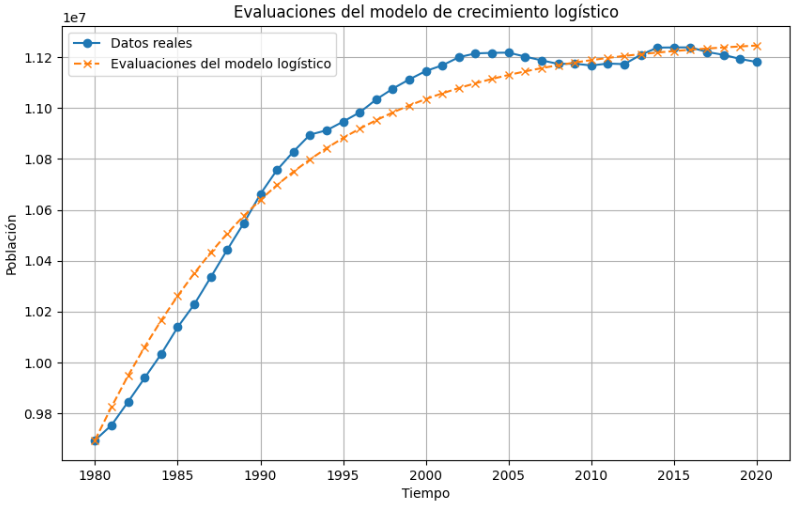
\includegraphics[height = 7cm]{img/real_vs_pred.png}
    \end{center}
\end{frame}

\begin{frame}{Predicción del modelo sin intervalos}
    \begin{center}
        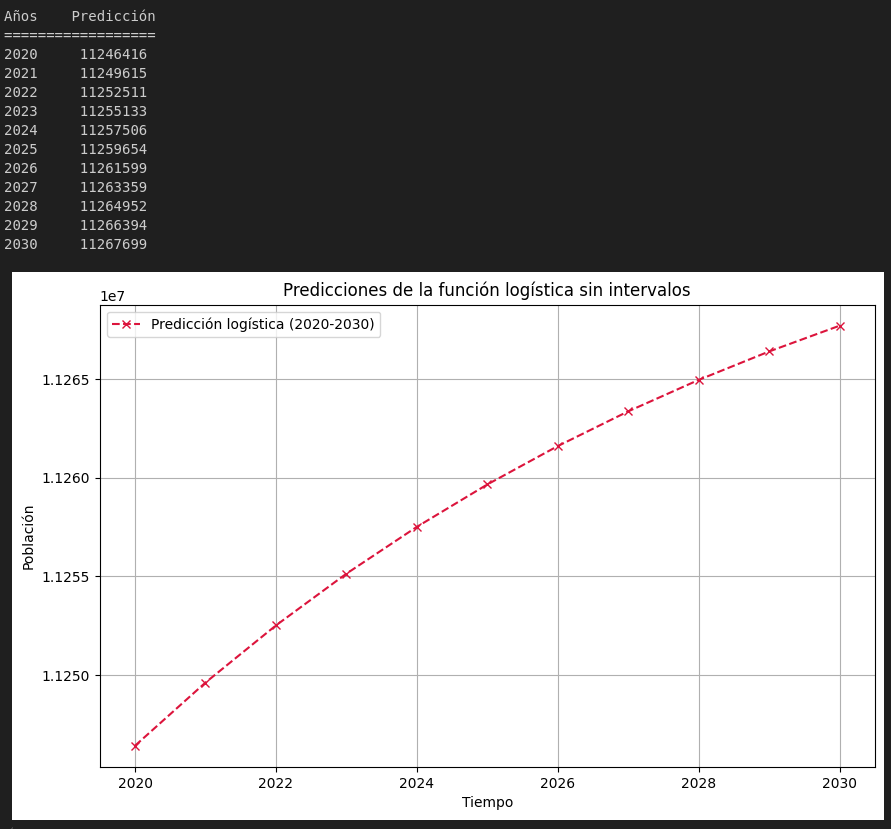
\includegraphics[height = 7cm]{img/graph_sin_intervalos.png}
    \end{center}
\end{frame}

\begin{frame}{Predicciones hasta el 2030}
    \begin{figure}[h!]%
		\begin{center}
			\begin{tabular}{|c|c|c|} \hline
            Años	& Predicción    \\ \hline
            2020 	& 11246416      \\ \hline
            2021 	& 11249615      \\ \hline
            2022 	& 11252511      \\ \hline
            2023 	& 11255133      \\ \hline
            2024 	& 11257506      \\ \hline
            2025 	& 11259654      \\ \hline
            2026 	& 11261599      \\ \hline
            2027 	& 11263359      \\ \hline
            2028 	& 11264952      \\ \hline
            2029 	& 11266394      \\ \hline
            2030 	& 11267699      \\ \hline
            \end{tabular}
        \caption{Resultados del modelo sin intervalos \label{fig:ex}}
    \end{center}
\end{figure}
\end{frame}
\begin{frame}{DataFrame para intervalos de 5 años}
	\begin{figure}[h!]%
		\begin{center}
			\begin{tabular}{|c|c|c|} \hline
			 			& K 			& r 		\\ \hline
			0 			& 20442337054 	& 0.008  	\\ \hline
			1			& 340143106946 	& 0.003 	\\ \hline
			2			& 	  10660179	& -0.352 	\\ \hline
			3 			&   5105238279	&  0.000	\\ \hline
			4 			& 	2575174752	&  0.000 	\\ \hline
			5 			& 	   1223441	&  0.000	\\ \hline
			6 			& 	 999003076	&  0.000 	\\ \hline
			7 			& 	   1798999	&  0.000 	\\ \hline
			\end{tabular}
		\caption{Resultados del segundo modelo para el grupo de intervalos de 5 años \label{fig:ex}}
	\end{center}
\end{figure}
\end{frame} 

\begin{frame}{DataFrame para intervalos de 10 años}
    \begin{figure}[h!]%
        \begin{center}
            \begin{tabular}{|c|c|c|} \hline
                         & K 			& r 		\\ \hline
                0		 & 2059434657188& 0.009		\\ \hline
                1		 &10623571		& -0.135	\\ \hline
                2		 & 726227		& -0.000	\\ \hline
                3		 & 5837330070	& 0.000		\\ \hline
            \end{tabular}
        \caption{Resultados del segundo modelo para el grupo de intervalos de 10 años \label{fig:ex}}
        \end{center}
    \end{figure}
\end{frame} 

\begin{frame}{DataFrame para intervalos de 8 años}
    \begin{figure}[h!]%
        \begin{center}
            \begin{tabular}{|c|c|c|} \hline
                         & K 			& r 		\\ \hline
                0		 & 2055969070415& 0.009		\\ \hline
                1		 & 10396071	    & -0.167	\\ \hline
                2		 & 10981262	    & -0.209	\\ \hline
                3		 & 1000853	    & 0.000		\\ \hline
                4		 & 11251162	    & 0.022		\\ \hline
            \end{tabular}
        \caption{Resultados del segundo modelo para el grupo de intervalos de 8 años \label{fig:ex}}
        \end{center}
    \end{figure}
\end{frame} 

\begin{frame}{Predicción del modelo en intervalos de 8 años}
    \begin{center}
        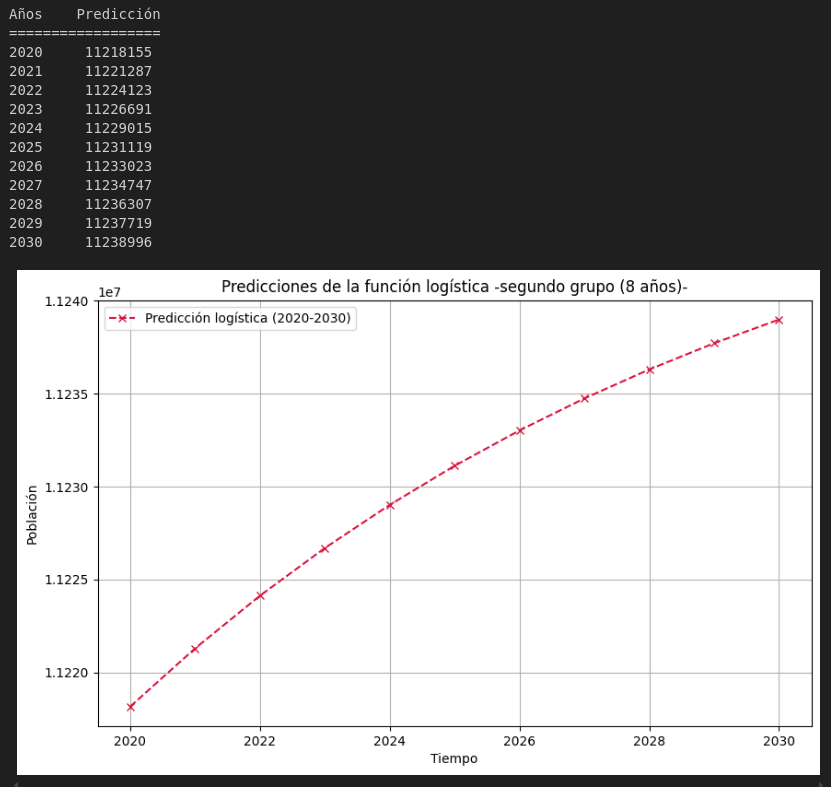
\includegraphics[height = 7cm]{img/df8_graph.png}
    \end{center}
\end{frame}

\begin{frame}{Predicciones hasta el 2030}
    \begin{figure}[h!]%
		\begin{center}
			\begin{tabular}{|c|c|c|} \hline
            Años	& Predicción		\\ \hline
            2020 	& 10548308		    \\ \hline
            2021 	& 10562666		    \\ \hline
            2022 	& 10576750		    \\ \hline
            2023 	& 10590563		    \\ \hline
            2024 	& 10604111		    \\ \hline
            2025 	& 10617398		    \\ \hline
            2026 	& 10630427		    \\ \hline
            2027 	& 10643205		    \\ \hline
            2028 	& 10655733		    \\ \hline
            2029 	& 10668018		    \\ \hline
            2030 	& 10680063		    \\ \hline
            \end{tabular}
        \caption{Resultados del modelo en intervalos de 8 años\label{fig:ex}}
    \end{center}
\end{figure}
\end{frame}

\begin{frame}{Predicción del modelo en intervalos de 8 años desde 1980 hasta 2030}
    \begin{center}
        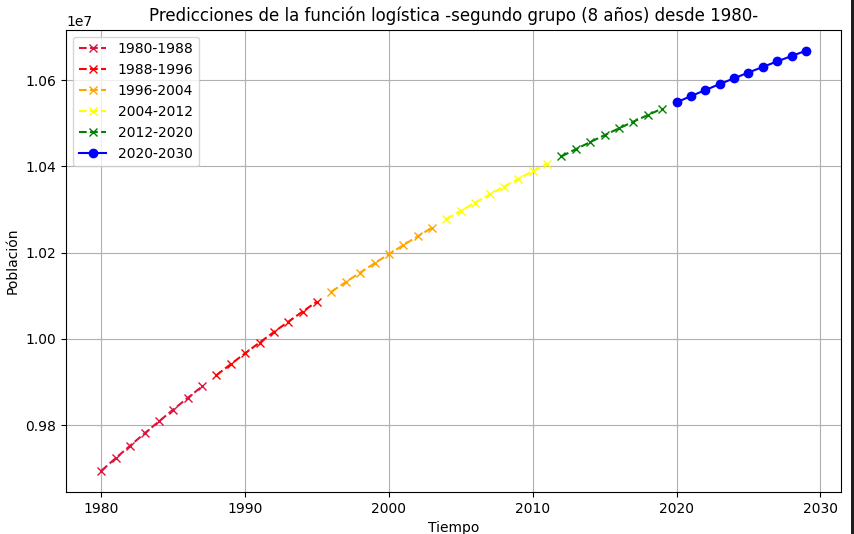
\includegraphics[height = 7cm]{img/prediccion.png}
    \end{center}
\end{frame}

\section{End}
\begin{frame}{Recomendaciones}
\begin{itemize}
    \item Mejorar el Modelo Matemático
    \item Ampliar la Base de Datos
    \item Validar y Refinar el Modelo
    \item Investigar Factores Externos
    \item Divulgar los Resultados
    \end{itemize}
    Estas recomendaciones buscan fortalecer el modelo actual, ampliar su alcance y utilidad, y contribuir al conocimiento demográfico de Cuba, teniendo en cuenta las particularidades observadas en el análisis inicial.
\end{frame}

\begin{frame}{Muchas gracias :)}
    \begin{center}
    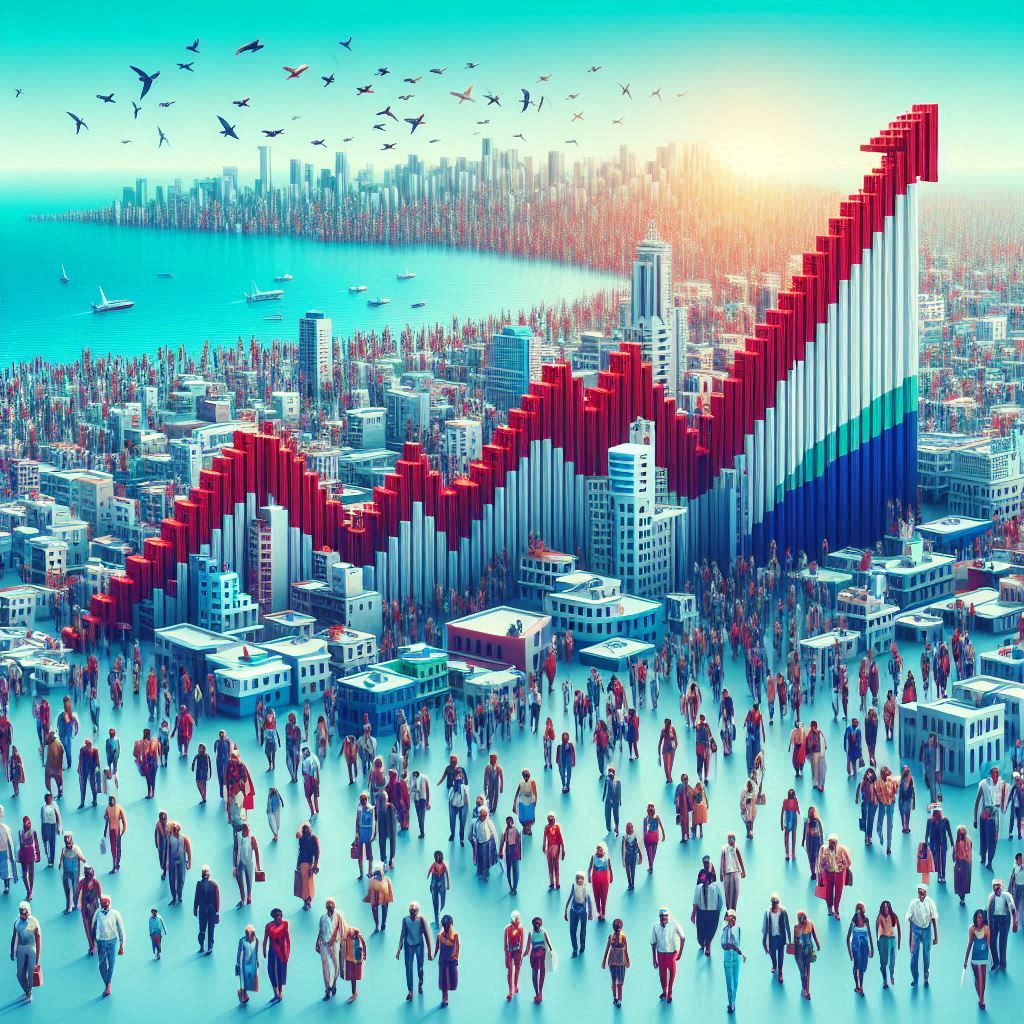
\includegraphics[height = 8cm]{img/cuba1.jpeg}
    \end{center}
\end{frame}

\end{document}